
\section{转换程序的设计}

\subsection{需求分析}

\newsavebox{\umluc}
\sbox{\umluc}{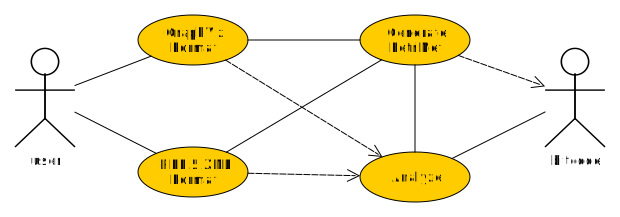
\includegraphics[width=12cm]{image/uml-usecase.pdf}}
\begin{figure}[!hbt]
\centering
\usebox{\umluc}
\caption{数据流分析Pass的用例图} \label{fig:umluc}
\end{figure}

本程序通过LLVM的组件opt调用。由opt的 \code{-load} 参数加载。
向opt传入 \code{-help} 参数时,必须能够正确显示本程序的标识。
向opt传入本程序的标识时,必须能够正常启动本程序的功能。

程序需要解析LLVM生成的bitcode。并将解析的结果转换成为程序内部的图的数据结构。
这个图的数据结构就是已生成的随机Petri网的结构。

生成了随机Petri网的结构后,程序应当将它序列化,打印在文件里。
同时,对于功能兼容方面有这样的要求:用户可以选择将随机Petri网的数据结构序列化为GraphViz的dot格式,或者可用于PIPE5的xml格式。

生成的xml格式在PIPE5软件中必须可以编辑,这是随机Petri网分析的前提条件。


\subsection{概要设计}

\newsavebox{\umlclass}
\sbox{\umlclass}{\includegraphics[width=13cm]{image/uml-class.pdf}}
\begin{figure}[!hbt]
\centering
\usebox{\umlclass}
\caption{数据流分析Pass的类图} \label{fig:umlclass}
\end{figure}

程序相当于是一个LLVM的opt插件。在opt启动时,它会读取 \code{FunctionPass} 类中的静态变量 \code{ID},交给Pass管理器。
由管理器统一分配系统资源给每一个Pass,之后预处理输入的bitcode,并生成 \code{llvm::Module} 这个图结构。

opt开始遍历这个图结构,并视每次遇到子结构为一个事件。这个事件会触发opt执行各个Pass中的方法。
本程序会注册“\code{OnFunction}”这个事件。当opt每遇到一个代表函数的结构时,都会调用 \code{runOnFuntion} 方法,这也是本程序的入口函数。

本程序会进一步读取、分析这个由opt预处理好的图结构,从中找出数据流、数据依赖关系、程序分支 \cite{llvmmanual}。
之后整理这些分支,将它们重新生成为随机Petri网的结构。

为了保证clang与GCC编译器都可通过,程序加入了 \code{std::string} 的扩展 \code{to_string} 方法。
有些符号不会显示在最终结果中,为了简化这些符号处理,\code{str_util} 命名空间还加入了一个快速校验算法 \code{adler32}。
针对LLVM IR频繁使用的一系列命令则封装为 \code{LLVMUtil} 命名空间。

表 \ref{tab:fault} 给出了程序可能发生的问题,故障的严重性及解决方法。

\begin{table}[!hbt]
\centering
\caption{预计故障列表} \label{tab:fault}
\renewcommand{\arraystretch}{2.62}
\footnotesize
\begin{tabular}{llll}
\hline 故障 & 等级 & 推测 & 解决 \\ \hline
Segmentation Fault & 严重 & 程序本身设计不完整导致内存泄漏 & \makecell[l]{使用调试、日志的方式 \\ 寻找并修正错误} \\
LLVM API抛出未捕获异常 & 严重 & 程序错误地调用了LLVM API & 在抛出异常处的代码添加内容检查 \\
opt提示Pass注册多次并退出 & 严重 & 程序的链接时错误 & \makecell[l]{根据LLVM安装的方式与系统平台 \\ 正确使用编译参数} \\
生成的图点、边数量错误 & 较严重 & 程序逻辑不完整、算法不周全 & \makecell[l]{使用调试的方式 \\ 对照输入数据修正逻辑} \\
生成的图节点属性错误 & 中等 & 程序逻辑不完整、算法不周全 & \makecell[l]{使用调试的方式 \\ 对照输入数据修正逻辑} \\
生成的图边属性错误 & 中等 & 程序逻辑不完整、算法不周全 & \makecell[l]{使用调试的方式 \\ 对照输入数据修正逻辑} \\
无任何输出文件 & 轻度 & \makecell[l]{opt程序执行方法错误 \\ 输入文件格式不匹配} & \makecell[l]{检查输入数据 \\ 命令行选项与工作目录} \\
\hline
\end{tabular}
\end{table}

对表 \ref{tab:fault} 中的一项“opt提示Pass注册多次并退出”问题的说明:
这是一个已知的平台相关的问题。在macOS中的LLVM的安装方式与在Ubuntu中的安装方式不同,则链接时传入的参数有所不同。
macOS中编译LLVM Pass时需要显式链接LLVM的库,而Ubuntu中不需要。
当在Ubuntu中链接时也传入这些库时,虽然能链接成功,但会导致opt加载时出现重复注册的提示。
因此,如果出现这个问题,只需修改链接参数即可。

\subsection{详细设计}

\subsubsection{类 \code{Analyzer}}
在第 \ref{sec:dcfgconv} 节中的算法 \ref{alg:eg:dfgllvm} 中已经介绍了
类 \code{Analyzer} 的方法 \code{Analyze(llvm::Funtion\&)} 的核心算法,
其中的 $VarList.renameAll()$ 的具体实现指的就是类中的 \code{_merge} 方法。

实现这个算法时尤其要注意对各变量的正确存储。代码靠近底层,信息庞杂,易出错。
虽然LLVM平台已经扫清了很多障碍,但是鉴于研究对象是接近汇编的复杂语言,仍然要小心。

本类只做代码分析,不会进行任何输入输出操作,以防止出现过度藕合的现象。

\code{Analyze}:此方法实现了第 \ref{sec:dcfgconv} 节中介绍的算法 \ref{alg:eg:dfgllvm}(基于LLVM的数据流——随机Petri网的转换)。
在这一节中曾提到了,LLVM的分支排列顺序是良好的,能够做到在遍历其中一个基本块时不漏下任何分支。
这一点在实现此方法时应该更深层地考虑一下,是否存在特别的顺序导致破坏了这种可以在遍历的途中就能得到所有信息的优势。
所以,如果确实出现了这一点,可以将代码稍作修改,让代码先遍历一次所有的基本块,获取所有的分支信息后,再执行数据流——随机Petri网的转换算法。
因此,这一点可加入预计的故障列表。

\subsubsection{类 \code{AnalyzeToPNet}}
本类继承类 \code{Analyzer}。主要用于将类 \code{Analyzer}生成的随机Petri网数据结构序列化为PIPE5可读的xml格式。

本类会进行输入输出操作。会将序列化的结果保存在外部文件内。保存路径是opt程序的工作目录。

本类继承类 \code{llvm::FunctionPass}。重载父类的回调方法 \code{runOnFunction}。在opt存在相关选项时,由opt调用。
\code{runOnFunction} 方法是本类的入口函数。本类重载静态变量 \code{ID},是用于LLVM的Pass管理器的唯一识别号,
可用于在同一个动态链接库中开发多个Pass,表现在opt的行为上是多个编译器选项。
本类与类 \code{AnalyzeToDot} 共存,拥有不同的ID,可通过opt的编译器选项选择其中之一来执行。


\subsubsection{类 \code{AnalyzeToDot}}
本类继承类 \code{Analyzer}。主要用于将类 \code{Analyzer}生成的随机Petri网数据结构序列化为GraphViz可读的dot格式。

本类会进行输入输出操作。会将序列化的结果保存在外部文件内。保存路径是opt程序的工作目录。

本类继承类 \code{llvm::FunctionPass}。重载父类的回调方法 \code{runOnFunction}。在opt存在相关选项时,由opt调用。
\code{runOnFunction} 方法是本类的入口函数。本类重载静态变量 \code{ID},是用于LLVM的Pass管理器的唯一识别号,
可用于在同一个动态链接库中开发多个Pass,表现在opt的行为上是多个编译器选项。
本类与类 \code{AnalyzeToPNet} 共存,拥有不同的 \code{ID},可通过opt的编译器选项选择其中之一来执行。




\subsubsection{命名空间 \code{str_util}}
本命名空间提供开启了C++11标准的GCC仍然不支持的方法std::string::to_string(T)。
提供此方法后,程序使用clang或GCC均可编译通过。

本命名空间提供了简单快速哈希算法adler32。如果有绘制子图的需求,可以简化字符串的处理。
具体为,使用哈希数字代替包含大量特殊符号的函数名写入序列化后的文件,但不影响用户使用。

\code{to_string}:为GCC设计的扩展方法,是一个泛型函数。它以 \code{std::ostringstream} 为核心。
任何一个重载了对 \code{std::stream} 的输出操作的类型都可以由此函数方便地序列化为字符串。

\code{adler32}:计算一个缓冲区的哈希,并返回一个32位整数。

\code{adler32_str}:封装了 \code{adler32} 方法。返回的是由 \code{adler32} 返回的整数所转化成的字符串。




\subsubsection{命名空间 \code{LLVMUtil}}
本命名空间提供与LLVM平台和C++语言相关的常用工具的封装。

\code{GetVarName}:此方法允许用户获取LLVM指令的运算目标的寄存器的名称。
例如对于指令 $\%a = mul nsw i32 \%22, \%21$,此方法会获取第a号寄存器的名字。
如果目标寄存器在LLVM汇编代码中使用数字表示,则此名称不存在。

\code{GetVarDescript}:此方法允许用户获取完成的LLVM指令的描述,即以普通文本的形式获取当前指令的LLVM汇编代码。
所获取的字符串与 \code{clang -S -emit-llvm} 程序的输出结果一致。可以在指令难以分析的情况下通过此功能解析文本形式。

\code{DemangleName}:C++编译器为确保命名空间与函数重载功能的正常运行,会将函数名字修饰为唯一的标识符。
修饰后的名字非常不方便阅读,需要对其进行反修饰。此方法将经过了名字修饰的C++函数名复原为可读的文本形式。
例如,传入下面这个修饰后的函数名称:

\begin{lstlisting}
_ZNK3MapI1T3RefI1SE10ComparatorIS0_E9AllocatorE3hasERKS0_
\end{lstlisting}

此方法会返回这样的结果:

\begin{lstlisting}
Map<T, Ref<S>, Comparator<T>, Allocator>::has(T const&) const
\end{lstlisting}

\code{TypeToStr} 与 \code{InstToStr}:这两个方法分别获取LLVM的类型与指令的LLVM汇编文本表达形式。
方法 \code{GetVarDescript} 调用了 \code{InstToStr}。
